In this section we provide a brief background to Architecture-Driven Modernization (ADM) presenting the core ideas. Furthermore, this section describes the ADM standards, e.g., Knowledge Discovery Metamodel (KDM), Abstract Syntax Tree Metamodel (ASTM) and Software Metrics Metamodel (SMM). Finally, we  justify the need for a systematic review study in this research field.

\subsection{Architecture-Driven Modernization}

Nowadays, researchers have been shifted from the typical refactoring process to the so-called Architecture-Driven Modernization (ADM). ADM is the concept of modernizing existing systems with a focus on all aspects of the current systems architecture and the ability to transform current architectures to target architectures by using all principles of MDA~\cite[p.~60]{Ulrich:2010:IST:1841736}. Figure~\ref{horseshoe} shows the ADM modernization domain model where the left side of the horseshoe is the current state of a business architecture ``as-is'' and the right side is what we want to get after the modernization ``to-be''.


\begin{figure}[!ht]
\centering
  % Requires \usepackage{graphicx}
  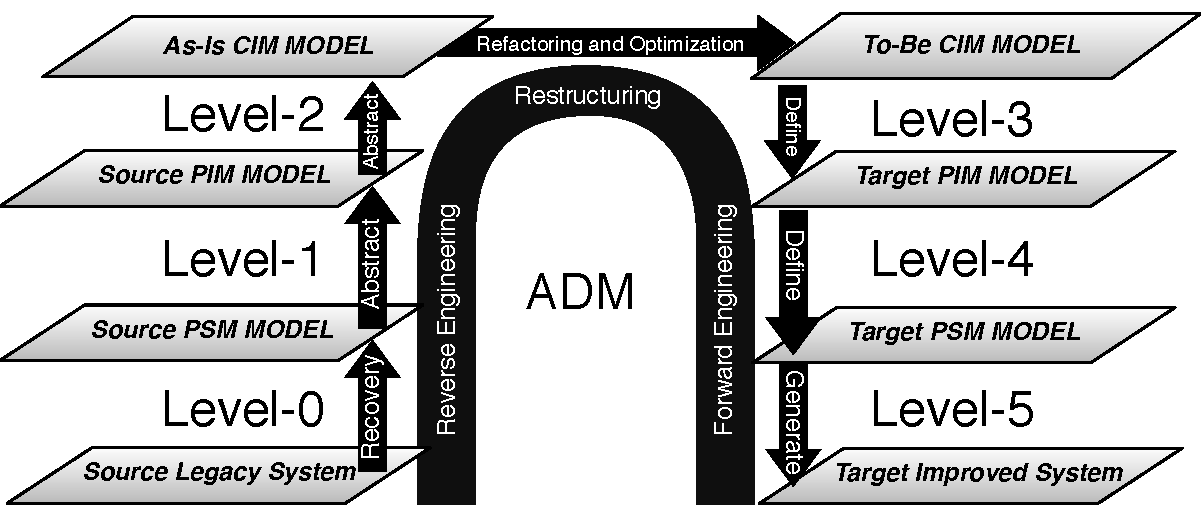
\includegraphics[scale=0.4]{figuras/Fonte_horse_shoe}
\caption{Modernization domain model (Adapted from Ulrich and Newcomb~\cite{Ulrich:2010:IST:1841736})}
\label{horseshoe}
\end{figure}

As can be seen in Figure~\ref{horseshoe} the horseshoe reengineering model has been adapted to ADM and it is nowadays known as horseshoe modernization model. As ADM uses the principles of MDA three kinds of models in the horseshoe are used, they are: (\textit{i}) PIM - \textbf{P}lataform \textbf{I}ndependent \textbf{M}odel which represents a view of the system from the platform independent viewpoint at an intermediate abstraction level, (\textit{ii}) PSM - \textbf{P}lataform \textbf{S}pecific \textbf{M}odel which constitutes a view of the system from the platform specific viewpoint at a low abstraction level, and (\textit{iii}) CIM - \textbf{C}omputational \textbf{I}ndependent \textbf{M}odel that represents a view of the system from the computational independent viewpoint at a high abstraction level. These models are used in the steps of the ADM process, i.e., Reverse Engineering, Restructuring, and Forward Engineering. In the first step, a reverse engineering is performed starting from the artifacts of the legacy system (source code, database, configuration files, etc) and a set of PSM are created. Next, refactoring and restructuring techniques can be applied on these models in order to solve problems found in the legacy system. Therefore, this step consist of a set of transformation from the input model (``as-is'') to obtain a target model (``to-be''). Finally, a forward engineering is carried out and the source code of the modernized target system is generated again. 


In order to perform such steps, ADM introduces several modernization standards: Abstract Syntax Tree Metamodel (ASTM), Knowledge Discovery Metamodel (KDM), Structured Metrics Metamodel (SMM), etc. The next subsections present more information about these standards:


%System Assurance \& Evidence, Software Quality and Business Architecture Standards. Nevertheless, in this paper we are especially interested in KDM, i.e., it is the key cornerstone of ADM and KDM owns a set of metamodel elements whose purpose is to represent implementation level program elements and their associations. The details of KDM are described as follows:

\subsubsection{Abstract Syntax Tree Metamodel - ASTM}

Abstract Syntax Tree Metamodel (ASTM) was established to represent software at a very granular level of procedural logic, data definition, and workflow composition. ASTM can provide this granular level of information to KDM (see Section~\ref{subsec:KDM}) to augment the KDM view of a system. As a standard, ASTM can stand alone and supports tools geared at the complete, functionally equivalent refactoring and transformation of a system from one platform and language environment to a target platform and language environment. ASTM is a model that represent software artifacts using data structures that represent the types of language constructs, its compositional relationships to other language constructs, and a set of direct and derived properties associated with each language construct. The ASTM is derived by analyzing software artifacts and provides a way to create a representation of those software artifacts. 

\begin{figure}[!ht]
\centering
  % Requires \usepackage{graphicx}
  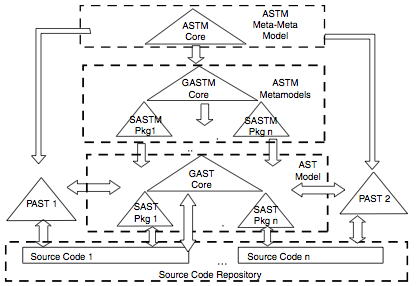
\includegraphics[scale=0.56]{figuras/ASTM}
\caption{ASTM modeling framework}
\label{ASTM}
\end{figure}

ASTM aims to facilitate exchanging software models in standard formats among tools. This ability of exchanging software models between tools is thanks to its attributes, they are: (\textit{i}) ASTM is language and platform independent, but can be extended as needed, (\textit{ii}) ASTM uses XMI formats for tool-based metadata exchange, \textit{iii} Generic Abstract Syntax Tree Metamodel (GASTM) represents a generic set of language modeling elements common across numerous languages. Language Specific Abstract Syntax Tree Metamodel (SASTM) represents particular languages such as Ada, C, FORTRAN, and Java, \textit{iv} Proprietary Abstract Syntax Tree Metamodel (PASTM) expresses ASTs for languages such as Ada, C, COBOL, etc., modeled in formats inconsistent with MOF, the GSATM, or SASTM. Figure~\ref{ASTM} represents the structure of the ASTM, including the SASTM, GASTM, and PASTM.

\subsubsection{Knowledge Discovery Metamodel - KDM}\label{subsec:KDM}

Knowledge Discovery Metamodel (KDM) is the key within set of standards~\cite{1686216}. KDM allows standardized representation of knowledge extracted from legacy systems by means of reverse engineering. KDM provides a common repository structure that makes possible the exchange of information about existing software assets in legacy systems. This information is currently represented and stored independently by heterogeneous tools focused on different software assets~\cite[p.~32]{Ulrich:2010:IST:1841736}. Figure~\ref{kdm} shows each of the varying views of the existing IT architecture represented by the KDM. For example, the build view, depicts system artifacts from a source, executable, and library viewpoint. Other perspectives include design, conceptual, data, and scenario views.

\begin{figure}[!ht]
\centering
  % Requires \usepackage{graphicx}
  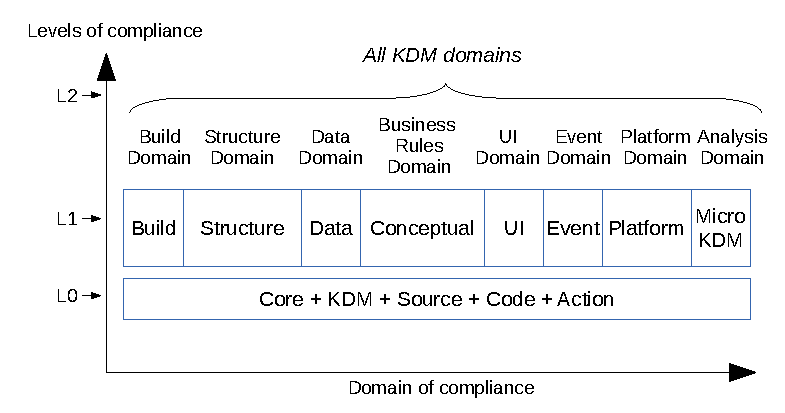
\includegraphics[scale=0.67]{figuras/kdm}
\caption{KDM domains of artifact representation (Adapted from Ulrich and Newcomb~\cite{Ulrich:2010:IST:1841736})}
\label{kdm}
\end{figure}

The Level 0 (L0) encompasses the Infrastructure and Program Elements Layer. Infrastructure Layer consists of the Core, kdm, and Source packages which provide a small common core for all other packages. Program Elements Layer consists of the Code and Action packages providing programming elements such as  data types, data items, classes, procedures, macros, prototypes, templates and captures the low level behavior elements of applications, including detailed control and data flow between statements. The Level 1 (L1) cover the Resource Layer which represents the operational environment of the existing software system. For example, the knowledge related to events and state-transition, the knowledge related to the user interfaces of the existing software system and the knowledge related to persistent data, such as indexed files, relational databases, and other kinds of data storage. The Level 2 (L2) cover the Abstraction Layer which represents domain and application abstractions. 

As we stated earlier, herein we are only interested in the Program Element Layer - more specifically  in the Code Package, which represents the code elements of a program and their associations. Therefore, it is important to dig a little deeper in this metamodel because it is mainly used by our approach in order to identify concerns. 

In a given KDM instance, each instance of the code meta-model element represents some programming language construct, determined by the programming language of the existing software system. Each instance of a code meta-model element corresponds to a certain region of the source code in one of the artifacts of the existing software system. In addition, the Code package consists of $24$ classes  and contains all the abstract elements for modeling the static structure of the source code. However, we are particularly interested in some of them. In Figure~\ref{fig:programLayer} is depicted a chunk of the Code package. It worth to notice that the more important metaclasses used herein are highlighted.

\begin{figure}[!ht]
\centering
  % Requires \usepackage{graphicx}
  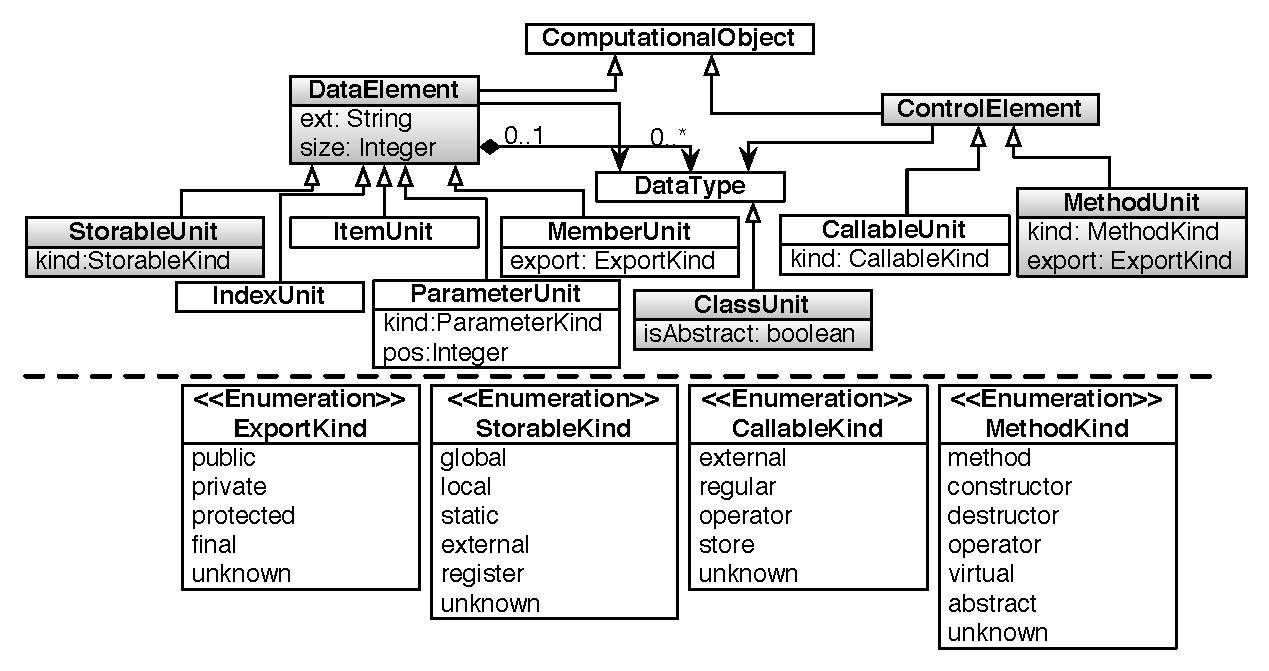
\includegraphics[scale=0.42]{figuras/ProgramLayer}
\caption{Chunk of the Code Package (OMG Group~\cite{OMGADM})}
\label{fig:programLayer}
\end{figure}

As can be seen in Figure~\ref{fig:programLayer} the root metaclass is \textit{ComputationalObject} which has two sub-metaclasses, i.e., \textit{DataElement} and \textit{ControlElement}. The former sub-metaclass, \textit{DataElement}, is a generic modeling element that defines the common properties of several concrete classes that represent the named data items of existing software systems, for example, global and local variables, record files, and formal parameters. \textit{DataElement} has five sub-metaclasses - \textit{StorableUnit}, \textit{IndexUnit}, \textit{ItemUnit}, \textit{ParameterUnit} and \textit{MemberUnit}. \textit{StorableUnit} is a concrete  sub-metaclass of the \textit{StorableElement} meta-class that represents variables of the existing software system. \textit{IndexUnit} class is a concrete subclass of the \textit{DataElement} class that represents an index of an array datatype. Instances of \textit{ItemUnit} class are endpoints of KDM data relations which describes access to complex datatypes. \textit{ParameterUnit} class is a concrete subclass of the \textit{DataElement} class that represents a formal parameter; for example, a formal parameter of a procedure. \textit{MemberUnit} class is a concrete subclass of the \textit{DataElement} class that represents a member of a class type. Finally, the latter, \textit{ControlElement} is a sub-metaclass that contains two sub-metaclasses - \textit{MethodUnit} and \textit{CallableUnit}. \textit{MethodUnit} element represents member functions owned by a \textit{ClassUnit}, including user-defined operators, constructors and destructors. The \textit{CallableUnit} represents a basic stand-alone element that can be called, such as a procedure or a function. As can be seen below the dashed line in Figure~\ref{fig:programLayer} there are also the following enumerations: ``\textit{ExportKind}'', ``\textit{StorableKind}'', ``\textit{CallableKind}'', ``\textit{MethodKind}'', which are sets os literals used as properties of the metaclasses.

\subsubsection{Structured Metrics Metamodel - SMM}

SMM (Structured Metrics Metamodel) provides a standard format to define metrics and to represent the measurement results. The main terms in SMM are measures and measurements. Measures are models which describes a way to calculate properties of software. For measurements can understand models containing results of applications of the metrics.

To apply SMM models in KDM models, a tool is needed to automate the process. The process occurs as illustrated in Figure X, the tool must receive an SMM model and a KDM model as input (KDM represents the software to be measured), then, after the measurements, other SMM model is generated as output and this model contains the results of the process.

There are some advantages in using SMM. It is advantageous because it is a standard, so, metrics defined in accordance with this metamodel can be tested, reused and shared. Furthermore, the use of a standard facilitates the development of compatible tools for automating the measurement process.

The SMM metrics can be of various types; direct, collective, binaries, etc. Direct metrics perform measurements of an index in a model. Collective metrics may measure multiple components and perform an operation with the result, for example; sum, average and others.
